\documentclass[varwidth=false, border=2pt]{standalone}

\usepackage{pgfplots}
\pgfplotsset{compat=1.17}
\usepackage{tikz}
\usepackage{nicefrac}
\pgfplotsset{every axis legend/.append style={
at={(0,0)},
anchor=north east}}

\begin{document}
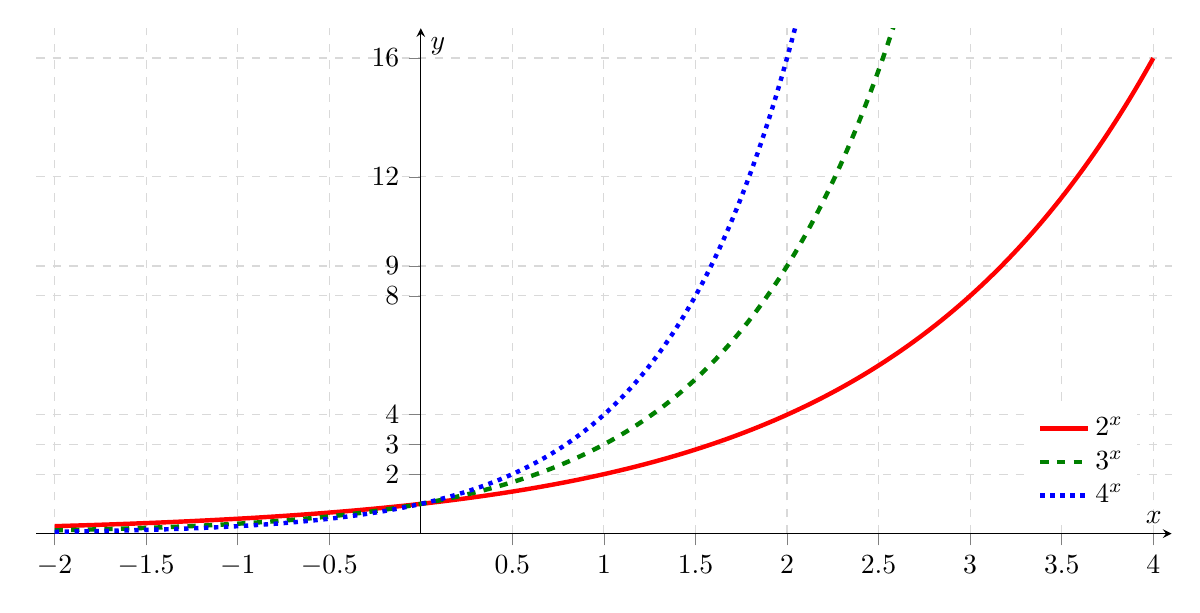
\begin{tikzpicture}
    \begin{axis}[
        axis x line=middle,
        axis y line=middle,
        grid = major,
        width=16cm,
        height=8cm,
        grid style={dashed, gray!30},
        xmin=-2.1,   % start the diagram at this x-coordinate
        xmax= 4.1,   % end   the diagram at this x-coordinate
        ymin= 0,     % start the diagram at this y-coordinate
        ymax= 17,    % end   the diagram at this y-coordinate
        xlabel=$x$,
        ylabel=$y$,
        ytick={0,2,3,4,8,9,12,16},
        yticklabels={0,2,3,4,8,9,12,16},
        legend cell align=left,
        legend pos=south east,
        legend style={draw=none},
        tick align=outside,
        enlargelimits=false]
      % plot the function
      \addplot[domain=-2:4, red, ultra thick,samples=500] {2^x};
      \addplot[domain=-2:4, green!50!black, ultra thick,dashed,samples=500] {3^x};
      \addplot[domain=-2:4, blue, ultra thick,dotted,samples=500] {4^x};
      \legend{$2^x$,$3^x$,$4^{x}$}
    \end{axis}
\end{tikzpicture}
\end{document}
